\documentclass[12pt]{article}
\usepackage[utf8]{inputenc}
\usepackage{amsmath}
\usepackage{mathrsfs}
\usepackage{amssymb}
\usepackage{amsfonts}

\DeclareMathOperator{\logit}{logit}
\DeclareMathOperator*{\argmax}{arg\,max}
\DeclareMathOperator*{\argmin}{arg\,min}

\usepackage[
    a4paper,
    left = 2.5cm,
    right = 2.5cm,
    top = 2.5cm,
    bottom = 2.5cm
]{geometry}

\usepackage{graphicx}
\usepackage[headings]{fullpage}
\usepackage{hyperref}
\usepackage{fancyhdr}
 %For aligned formulas
 \usepackage{IEEEtrantools}
\usepackage{listings} %Source code listings https://en.wikibooks.org/wiki/LaTeX/Source_Code_Listings

% \lstset{
%     language=R, %You can always set to another language
%     breaklines,
%     deletekeywords={category},
%     basicstyle=\ttfamily\footnotesize,
%     otherkeywords={!,!=,~,\$,*,\&,\%/\%,\%*\%,\%\%,<-,<<-},
%     literate={~}{$\sim$}1 {<-}{{$\gets$}}1
% }

\usepackage[
    backend=biber,
    style=apa,
    maxcitenames=2,
    mincitenames=1,
    sorting=ynt
    ]{biblatex}
\addbibresource{bibfile.bib}

\setlength{\headheight}{15pt}
\pagestyle{fancy}
\fancyhf{}
\rhead{Your Names} % Fill in your name
%\lhead{Bayesian Statistics \& Probabilistic Machine Learning---Project Report}
\rfoot{Page \thepage}


\begin{document}

\begin{titlepage}
        \centering % Center all text
        \vspace*{\baselineskip} % White space at the top of the page
        
        {\huge YOUR TITLE}\\[0.2\baselineskip] % Title
        
        
        \vspace*{\baselineskip}
        
        {\Large --- Project Report ---\\
          Advanced Bayesian Data Analysis\\[\baselineskip]} % Tagline(s) or further description
        \vspace*{\baselineskip}
        
        {\LARGE Eldaleona Odole \and Leonor Cunha \and Anarghya Murthy\\[\baselineskip]} % Editor list  
        
        \vspace*{\baselineskip}

        \vfill
        
        \today \par % Location and year
        
        \vspace*{\baselineskip}

        {\itshape TU Dortmund University\par} % Editor affiliation
    \end{titlepage}

\clearpage

% \section{Template}
% This is a template for the project report in the course Advanced Bayesian Data Analysis.
% Fill in your title and names for the title page and header and follow the general structure. You don't have to use multiple chapters or sections at all for this short report, but if you do, don't go further than subsections--- \textcite{feynman1963lnphysics} didn't need to\ldots

% Some examples on how to use \LaTeX{} are shown below. If you want to reference something, you can do it as so:
% \textcite{mcelreath2016statistical}.

% \subsection{Images}
% \begin{figure}
%     \begin{center}
%     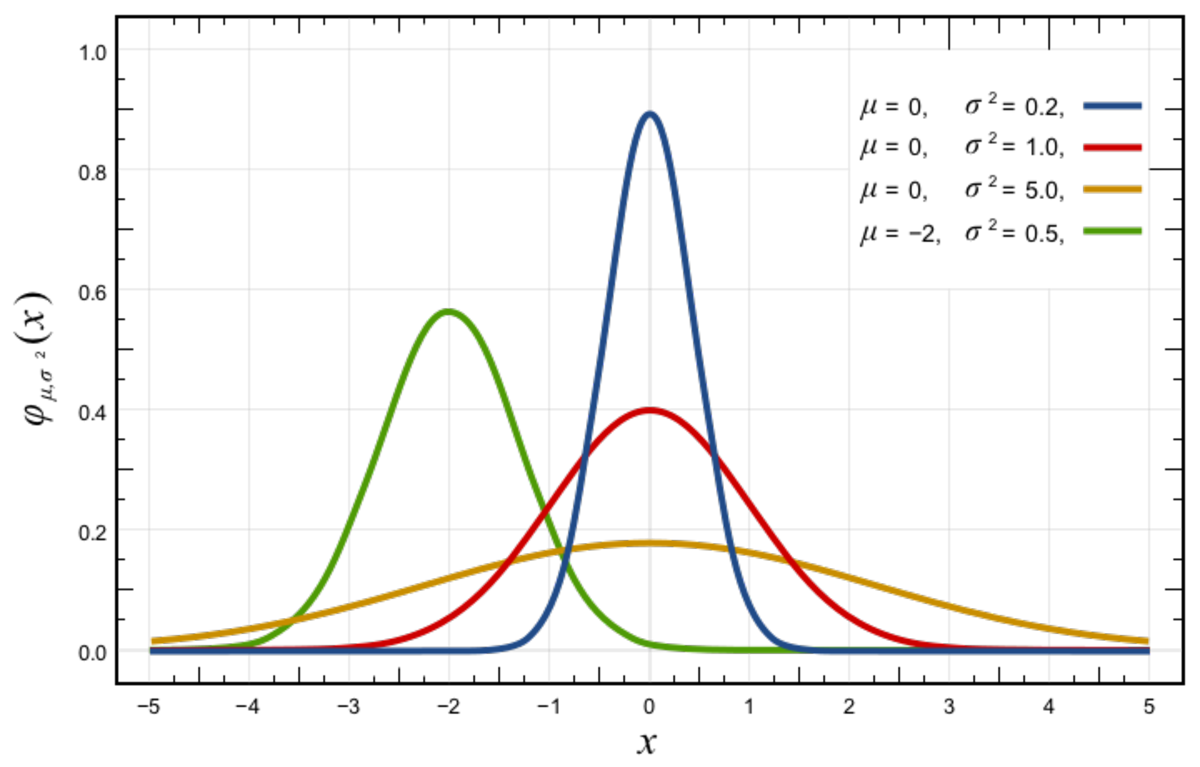
\includegraphics[width=0.5\textwidth]{figures/Normal_Distribution_PDF.pdf} %try to never force a figure placement
%     \caption{Probability density function for the Normal distribution. The red curve is the standard normal distribution. [By Inductiveload - self-made, Mathematica, Inkscape, Public Domain, \url{https://commons.wikimedia.org/w/index.php?curid=3817954}]}
%     \label{fig:normal_sample}
%     \end{center}
% \end{figure}

% This is an example for how to insert images into your document. When talking about a figure, you should always point out which one you mean, i.e., ``As you can see in Figure~\ref{fig:normal_sample}.''

% \subsection{Tables}
% A table has a caption \textit{above} the table as in Table~\ref{tab:my_label}.

% \begin{table} %You can place [h] immediately after \begin{table} to force the placement of the table. Generally speaking never do that---LaTeX usually places them in a sane way!
%     \centering
%     \caption{My caption.}
%     \label{tab:my_label}
%     \begin{tabular}{c|l} % l, r, and c justified inside cells.
%         \hline
%          Poisson & $\lambda$ \\ % Always end a line with \\
%          Normal &  $\mu$ and $\sigma$\\ 
%         \hline
%     \end{tabular}
% \end{table}

% \subsection{Formulas}
% This is a small example for how to include formulas into your document. $a^2 + b^2 = c^2$ will inline a formula, while
% $$c \leq a + b$$
% will give the formula its own line.

% \subsection{Formulas}
% You also might want to write out models:

% {\footnotesize % you align formulas using & 
% \begin{IEEEeqnarray*}{rCl}
% \mathrm{L}_i & \sim & \mathrm{Binomial}(n_i,p_i)\\
% \mathrm{logit}(p_i) & = & \alpha_{\mathrm{SUBJECT}[i]} + (\beta_P + \beta_{PC}C_i)P_i\\
% \alpha_{\mathrm{SUBJECT}} & \sim & \mathrm{Normal}(0,10) \\
% \beta_P & \sim & \mathrm{Normal}(0,10)\\
% \beta_{PC} & \sim & \mathrm{Normal}(0,10)
% \end{IEEEeqnarray*}
% }


% \subsection{Source code}
% Of course, formatting source code is always nice.
% \begin{lstlisting}
% m <- map(
%     alist(
%         height ~ dnorm(mu, sigma),
%         mu <- a + b*weight,
%         a ~ dnorm(0, 100),
%         b ~ dnorm(0, 10),
%         sigma ~ dunif(0, 50) 
%     ), 
%     data=d2)
% \end{lstlisting}

% \subsection{Math fonts}
% Different math fonts are also available to you:

% $\mathrm{ABCDE abcde 1234}$

% $\mathit{ABCDE abcde 1234}$

% $\mathnormal{ABCDEabcde1234}$

% $\mathcal{ABCDE abcde 1234}$

% $\mathscr{ABCDE abcde 1234}$

% $\mathfrak{ABCDE abcde 1234}$

% $\mathbb{ABCDE abcde 1234}$

\section{Introduction}

Every two years the United States elects 435 officials to the House of Representatives. The 435 House seats are allocated roughly proportional to population with additional constraint that each state must have at least one seat in the House of Representatives. However, despite being roughly equivalent in population size, the characteristics of voters living in each district varies greatly by district. 
Although technically a multiparty system, the U.S. is often called a two party system due to the domination of Democrats and Republicans at all levels of govenrment (cite). These parties dominate because political candidates are only required to get a plurality of votes, of which the two largest parties often reach. Additionaly would be third-party voters, will often vote for one of the two major parties so ensure their voice is heard, rather than using thier vote on a candidate who will likely not win (cite). Within our dataset, there are no districts represented by a third-party candidate and as such we often refer to the U.S. as being a two party system.  The association between a voters demographics (gender, age, education etc.) and their propensity to vote for either a democratic or republican candidates is a topic of extensive study. However, little is known about the relationship between voting outcomes and the voters environment.  In a very general sense, conventional wisdom says that cities tend to be more “blue”, meaning voters in large cities tend to vote for democrats. Our project is focused on characterizing this relationship more concretely. 
To answer our question about the nature of the relationship between urbanizaiton and partisan voting outcomes, we choose to investigate the 2022 House Election. This election takes places during a non-presidential year, which may cause additonal effects, this election also takes place most recently after the 2020 Census, allowing us to use the most recently available demographic data. 
Within this report we combine demographic data and urbanization data into a logistic regression model to predict the district voting outcomes of the 2022 House Election. The parameters 
% Previous attempts? 


\section{Dataset}


Our dataset was made by combining three independent datasets related to the 2022 House election. The first dataset is the publically available urbanization dataset published by fivethirty eight from which we incorporate the variables urbanization index  and (urban) grouping into our final dataset \cite{urbanizationdataset}. From the description of the dataset: "The urbanization index is calculated as the natural logarithm of the average number of people living within a five-mile radius of every census tract in a given district, based on a weighted average of the population of each census tract. The population of a census tract is according to 2020 census data. This provides a numerical value for how urban or rural a district is. " \cite{urbanizationdataset}. The urbanization dataset was put together by FiveThirtyEight as part of their analysis  \textit{The Republican Path To a House Majority Goes Through The Suburbs} which gave election predictions leading up to the 2022 U.S. Congressional Eleciton \cite{538urbanizationarticle}. 
% maybe add something about this analysis? 

The second dataset used in our analysis the Election Results Dataset from FiveThirtyEight \cite{electionresultsdataset}. It is a continuously updated repository of United States Govenor, Congressional and Presidential elections. As this dataset includes all elections going back to 1998, we only used a subset of the data relevant to the 2022 House Election. From this dataset we used the party, state, and winner variables. 

The third data used in our analysis is a subset of the 2022 American Commuity Survey Data. The American Community Survey is a yearly survey collecting information about the occupations, education attainment, income and other demographic information carried out by the United States Census Bureau. The United States Census Bureau provides an online tool to access its extensive survey database, which can then be filtered and refined for further analysis. For our analysis we used the following variables for each House district; 



\subsection{Data Cleaning}



\printbibliography

\end{document}
